%####################################################################################################################################################
% FYS4580 PROJECT REPORT
%####################################################################################################################################################

\documentclass[twocolumn,a4paper,10pt]{article}

\usepackage{graphicx}
\usepackage{amsmath}
\usepackage{slashed}
\usepackage{enumerate}
\usepackage{hyperref}
% \usepackage{caption}
% \usepackage{subcaption}


% Use all allowed space
\addtolength{\hoffset}{-0.5cm}
\addtolength{\textwidth}{1.0cm}
\addtolength{\voffset}{-1.5cm}
\addtolength{\textheight}{3cm}
\setlength{\columnsep}{0.5cm}

\author{Kevin Cappa \\ University of Oslo}

\title{{\huge FYS4580 - Semester Project Fall 2024} \\ 
        \noindent\rule[5pt]{12cm}{0.4pt} \\
        From Fuel Pin Cell to Reactor Core Design of APWRs \\
        A 13-Month Cycle Depletion Simulation with OpenMC} %Anatomy

\begin{document}

%####################################################################################################################################################
% ABSTRACT
%####################################################################################################################################################

\twocolumn[
\begin{@twocolumnfalse}
  \maketitle
  \begin{abstract}
    In this report we will discuss the basic structure of an advanced pressurized water reactor (APWR) for a model simulation in OpenMC. The report will follow the overarching structure of the FYS4590 project description for the Fall semester 2024. After defining the materials and the geometry of the reactor we will delve deeper in to the underlaying reactor physics of the model through a depletion calculation and laslty we will discuss the obtained results.
  \end{abstract}
  \vspace{5mm}
\end{@twocolumnfalse}
]

%####################################################################################################################################################
% ESSAY
%####################################################################################################################################################

%####################################################################################################################################################
% 1 - INTRODUCTION
%####################################################################################################################################################

\section{Introduction}

The main scope of this project report is to give a thourough, albeit simple, overview of introductory reactor physics applied to a rudimentary reactor core simulation. We will show how to build a modern advanced pressurized reactor (APWR) from its basic building block, the pin cell, to its outermost layer, the reactor pressure vessel, and give a brief discussion on how such a reactor differ from the usual pressurized water reactor (PWR). We will go into detail about the composition of the different pin cells that constitute the APWR, the assembly and core geometry and finally go through a depletion calculation in section~\ref{sec:Simulation}. This will aid us in discussing key points about criticality, fuel burnup, the conversion of uranium-235 to plutonium-239 in the reactor core, in addition to see how the chosen geometry and composition influences the the different factors in the four/five factors formula. This setup has been inspired by a paper published by K. Seki et.al. at the 2003 IAEA/INIS ``International conference on global environment and advanced nuclear power plantsonference" organized by the Atomic Energy Society of Japan in Kyoto, Japan~\cite{APWR}. Although, due to the usual lack of detailed information in publicly published papers on nuclear reactor cores' designs, we decided to extend the geometry by implementing a typical assembly configuration for reactors containing burnup fuels like gadolinia~\cite{BurnupFuel}. In the end a concise discussion of the pros and cons of this type of reactors will be explored in section~\ref{sec:Discussion} and lastly, we will give an outline of the accuracy of our model and simulation, possibles improvements and furhter developments in section~\ref{sec:Conclusion}. The source code for the simulation can be found in the author's GitHub folder~\cite{GitHub}.

%####################################################################################################################################################
% 2 - SIMULATION
%####################################################################################################################################################

\section{OpenMC Simulation}
\label{sec:Simulation}

\subsection{Materials and Geometry}

The basic building block of a nuclear reactor design is the fuel pin cell. In our case, for the chosen reactor design of the proposed japanese APWR, we have several kinds of pin cells inside the reactor core. Firstly we built the fuel pin cell, made of three concentric cyslindrical layers. The innermost cylinder is the fuel pellet, composed of uranium dioxide ($UO_2$), with a 4.8\% $^{235}_{92}U$ enrichment, and has a radius of 4,25 mm and is 36,6 mm tall. The next layer has a thickness of 0.2 mm and is filled with helium gass. This is done in order to accomodate for the fuel pellet thermal expansion. The outermost layer is a 3 mm thick cladding made of zyrcaloy-4, an alloy made up of 98.5\% zyrconium $(_{40}Zr)$ and 1.5\% tin $(_{50}Sn)$. The fuel pin cell is immersed in a box containing borated water, in this case is a 1\% boric acid ($B(OH)_3$) with 10\% boron $^{10}_{5}B$ concentration, in a light water suspension. This setup can be seen in Fig.~\ref{fig:fuelpinxy} and Fig.~\ref{fig:fuelpinyz}, where the uranium dioxide is colored in neon green, the helium is yellow, the zircaloy is light gray and the borated water is deep blue.

\newpage

\begin{figure}[ht]
  \centering
  \includegraphics[width=0.4\textwidth]{../Pictures/Fuelrods_plot_xy.png}
  \caption{Top view of the fuel pin cell.}
  \label{fig:fuelpinxy}
\end{figure}

\begin{figure}[ht]
  \centering
  \includegraphics[width=0.4\textwidth]{../Pictures/Fuelrods_plot_yz.png}
  \caption{Side view of the fuel pin cell.}
  \label{fig:fuelpinyz}
\end{figure}

\begin{figure}[ht]
  \centering
  \includegraphics[width=0.4\textwidth]{../Pictures/Burnablefuelrods_plot_xy.png}
  \caption{Top view of the burnable fuel pin cell.}
  %\label{fig:y equals x}
\end{figure}

\begin{figure}[ht]
  \centering
  \includegraphics[width=0.4\textwidth]{../Pictures/Burnablefuelrods_plot_yz.png}
  \caption{Side view of the burnable fuel pin cell.}
  %\label{fig:three sin x}
\end{figure}

\begin{figure}[ht]
  \centering
  \includegraphics[width=0.4\textwidth]{../Pictures/Controlrods_plot_xy.png}
  \caption{Side view of the control pin cell.}
  %\label{fig:y equals x}
\end{figure}

\begin{figure}[ht]
  \centering
  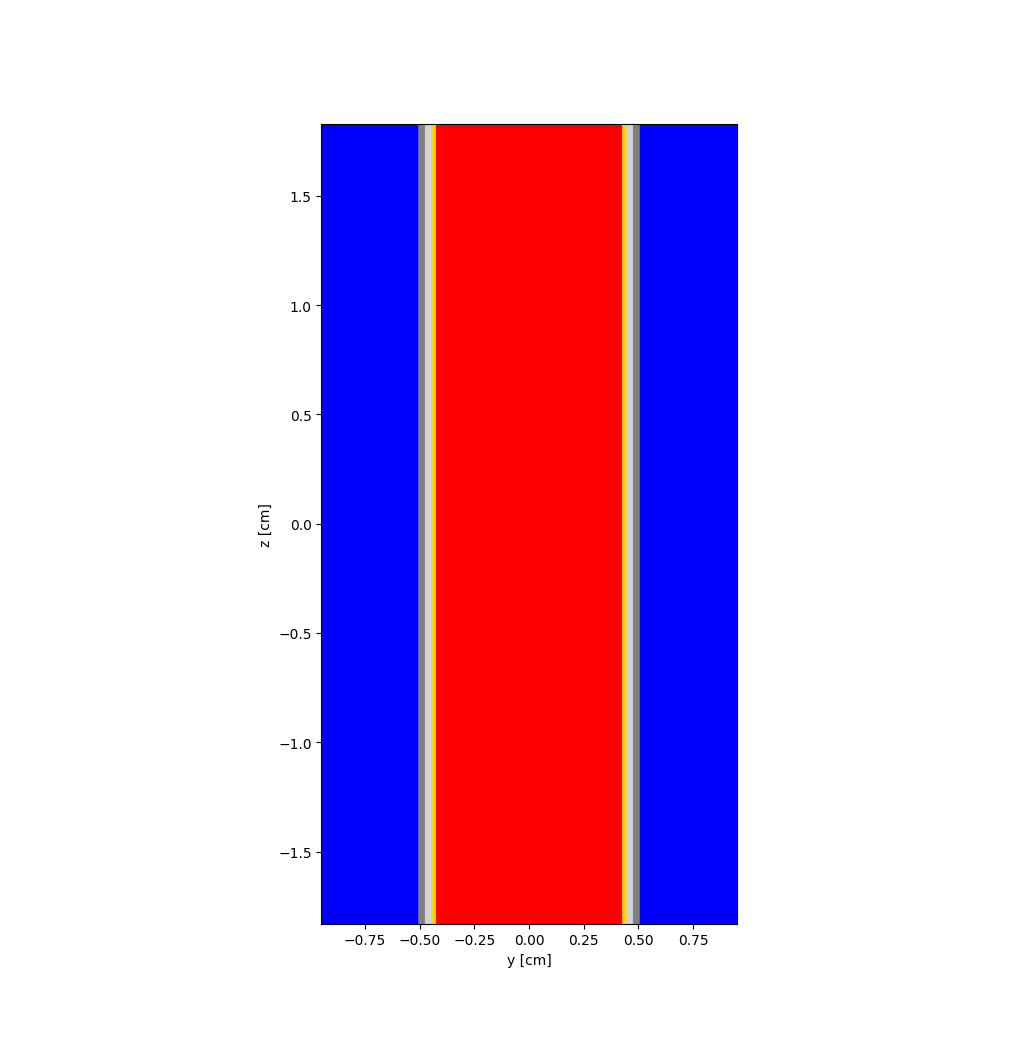
\includegraphics[width=0.4\textwidth]{../Pictures/Controlrods_plot_yz.png}
  \caption{Side view of the control pin cell.}
  %\label{fig:three sin x}
\end{figure}


\subsection{Tally Arithmetics}

\subsection{Depletion}

\subsection{Results}


%####################################################################################################################################################
% 3 - DISCUSSION
%####################################################################################################################################################

\section{Discussion}
\label{sec:Discussion}

Lorem ipsum dolor sit amet, consectetur adipiscing elit. Duis convallis vehicula metus in pretium. Nulla tincidunt lacus interdum feugiat tincidunt. Sed tincidunt, libero ac convallis semper, lectus diam congue nunc, id interdum ipsum lorem nec leo. Integer rutrum volutpat laoreet. Nullam vehicula leo eget metus ullamcorper aliquet. Vestibulum felis dui, auctor ut egestas sit amet, finibus quis eros. Ut vitae turpis eget dui vestibulum dapibus. Vivamus vitae facilisis enim. Phasellus efficitur odio quis felis ornare, nec congue risus consequat. Curabitur sapien massa, rhoncus vel arcu rhoncus, fermentum commodo augue. Donec eros nulla, fermentum non facilisis eu, scelerisque at dolor. Donec et vulputate augue, in pulvinar libero. Vivamus sit amet pulvinar sapien, non cursus nulla. Aliquam ut risus commodo libero tristique suscipit ac in odio.

Nulla euismod nisi sed nulla finibus sodales. Curabitur quis rhoncus urna. Donec sed lectus eget est commodo malesuada. Nunc pulvinar risus in tortor maximus, vehicula hendrerit turpis feugiat. Phasellus maximus risus dui, ut posuere est rutrum at. Fusce lacus neque, viverra a ex sed, dapibus scelerisque dui. Donec sed erat consectetur risus commodo pellentesque vel eu diam. 

%####################################################################################################################################################
% 4 - CONCLUSION AND FURTHER DEVELOPMENTS
%####################################################################################################################################################

\section{Conclusion and Further Developments}
\label{sec:Conclusion}

Lorem ipsum dolor sit amet, consectetur adipiscing elit. Duis convallis vehicula metus in pretium. Nulla tincidunt lacus interdum feugiat tincidunt. Sed tincidunt, libero ac convallis semper, lectus diam congue nunc, id interdum ipsum lorem nec leo. Integer rutrum volutpat laoreet. Nullam vehicula leo eget metus ullamcorper aliquet. Vestibulum felis dui, auctor ut egestas sit amet, finibus quis eros. Ut vitae turpis eget dui vestibulum dapibus. Vivamus vitae facilisis enim. Phasellus efficitur odio quis felis ornare, nec congue risus consequat. Curabitur sapien massa, rhoncus vel arcu rhoncus, fermentum commodo augue. Donec eros nulla, fermentum non facilisis eu, scelerisque at dolor. Donec et vulputate augue, in pulvinar libero. Vivamus sit amet pulvinar sapien, non cursus nulla. Aliquam ut risus commodo libero tristique suscipit ac in odio.

Nulla euismod nisi sed nulla finibus sodales. Curabitur quis rhoncus urna. Donec sed lectus eget est commodo malesuada. Nunc pulvinar risus in tortor maximus, vehicula hendrerit turpis feugiat. Phasellus maximus risus dui, ut posuere est rutrum at. Fusce lacus neque, viverra a ex sed, dapibus scelerisque dui. Donec sed erat consectetur risus commodo pellentesque vel eu diam. 

%####################################################################################################################################################
% REFERENCES
%####################################################################################################################################################

\small
\bibliography{Project}{}
\bibliographystyle{JHEP}
\begin{thebibliography}{}
% \raggedright
\bibitem{APWR}
K.~Seki, T.~Tanaka, Y.~Matsuura, \textit{Core and Fuel Design of APWR}, (GENES4/ANP2003,
Paper 1099,  International conference on global environment and advanced nuclear power plants, (p. 1675). Japan: Atomic Energy Society of Japan, Sep. 15-19, 2003,\\ Kyoto, JAPAN. IAEA INIS)
\url{https://inis.iaea.org/search/searchsinglerecord.aspx?recordsFor=SingleRecord&RN=36011909}

\bibitem{DocumentationPinCell}
OpenMC documentation on ``\textit{Tally Arithmetics}":\\
\url{https://docs.openmc.org/en/v0.11.0/examples/tally-arithmetic.html}

\bibitem{DocumentationDepletion}
OpenMC documentation on ``\textit{Pin Cell Depletion}":\\
\url{https://docs.openmc.org/en/v0.12.2/examples/pincell_depletion.html}

\bibitem{BurnupFuel}
K. Hesketh, \textit{Material Properties/Oxide Fuels for Light Water Reactors and Fast Neutron Reactors}, Comprehensive Nuclear Materials (2012)\\
\url{https://www.sciencedirect.com/topics/earth-and-planetary-sciences/gadolinium}

\bibitem{GitHub}
Author's GitHub repository for OpenMc simulation source code:\\
\url{https://github.com/KevinCappa/FYS4580_Project.git}

\end{thebibliography}

\end{document}

%####################################################################################################################################################
% END
%####################################################################################################################################################